\documentclass[version=last,fontsize=13pt]{scrartcl}

\usepackage{pdfpages}
\usepackage{graphicx}

\usepackage{indentfirst}

\usepackage{titlesec}
\usepackage{caption}

\titlespacing*{\section}{0pt}{3ex}{3ex}
\titlespacing*{\subsection}{0pt}{1.5ex}{1.5ex}
\titlespacing*{\subsubsection}{0pt}{1.5ex}{1.5ex}

\usepackage[margin = 0.8in]{geometry}

%my own paragraph for which the text that follows starts on a new line
\newcommand{\myparagraph}[1]{\paragraph{#1}\mbox{}\\}

% dont number sections
% \setcounter{secnumdepth}{0}

\usepackage{wrapfig}
\usepackage{float}

\usepackage{caption}
\usepackage{subcaption}

\usepackage{tabularx}
\usepackage{appendix}

\usepackage{caption}
\usepackage{subcaption}
\usepackage{hyperref}


\begin{document}

\begin{titlepage}
	\begin{center}	
		
\includegraphics[width = 5cm,height = 1.5cm]{./imgs/uws_logo.png}\\[5cm]

	{ \huge \bfseries %
		How can online learning companies use mobile technology to expand their market and generate new revenue?\\ \Large 
}
	\vspace{2cm}
	
	{\huge
		Part 2 
	}

	\vspace{2cm}			
			

			
		\begin{flushright}
				\large Student:\\
				Marius-Lucian Olariu\\[1cm]
		\end{flushright}
		
	
		\begin{flushleft}
			 \large
				Supervisor: \\
				Dr. Mark Stansfield \\[1cm]
		\end{flushleft}
		
	\vspace{2cm}	
	
		
		\vfill

			{\large {Paisley \\ 2019}}
		\end{center}
\end{titlepage}

\renewcommand{\labelenumi}{\roman{enumi}}

\newpage

\tableofcontents

\newpage

\listoffigures

\newpage

\section{Market Analysis}
	In the following lines, the author is going to analyze the mobile applications of the first two big players on the online learning market, namely, Coursera and edX. Both apps have the same target audience (mainly professionals), however, Coursera's app has to support a larger number of users.\\

	\subsection{Coursera}
		\subsubsection{Purpose and target audience}		   
		Coursera was founded by two professors from Standford University in order to teach a larger number of learners than it would have been possible in an on-site setting. The mobile \textbf{app}lication (app) supports the purpose of the organization by making the product (the courses) available "anywhere" with 20\% of the learners completing entire courses just through the mobile app (Samuelson, 2017).\\
		\indent
		The courses on Coursera contain university-level learning materials thus anyone above 18 years old who has high-school level knowledge can take them. Due to the fact that for each course one could receive a certification which can be uploaded on employment-oriented services like Linkedin, Coursera is very appealing to professionals who look for career advancement.\\ 
		\indent
		As can be observed in the Google Play description of the app the purpose of the app is to provide learning flexibility "Learn anywhere" and the main target audience is professionals who look  to advancement in their career (Coursera Android app, 2014).

		\subsubsection{Functionality}
		The app provides 5 main functionalities named: Explore, Recommended, Learn, Downloads and Profile. Please see Figure~\ref{courseraApp} for a visual depiction of the screen containing the Learn feature  and Appendix A for screenshots of the other features screens. The application is divided in sections using bar items that help the user to navigate between app features. The content of the application is synched with the Coursera webpage so that the user can freely change between the two modes of accessing the courses materials. In the following lines, each feature is going to be presented.

		\myparagraph{Learn}
		\indent
		Under this section all the courses to which a user is enrolled are shown. For each course, there is present a progress bar showing an estimate of how much work needs to be done to finish it. For each course the user can receive notifications regarding deadlines or set study reminders on specific weekdays and hours. Users can add also notes to videos, though, this feature is available only on iOS application. When the user picks one course to study from the courses to which he is enrolled the app will take him to another screen dedicated for that course. Usually the course view is structured in other 5 sections: Home (contains course materials: lectures slides, videos and questionnaires), Forums (discussions structured per week of study), Resources (additional materials, frequent asked questions), Grades (for each week of study an assignment is graded) and Messages (contains information about the course from course teachers). The \textit{learn} feature is avaliable only in online mode, thus when the user does not have an Internet connection he is directed to Downloads feature.

		\myparagraph{Downloads}
		\indent
		In order to provide greater flexibility the apps allows one to download the course materials (lecture slides, videos, quizzes) and access them offline. The course materials can be downloaded per week of study. Moreover, the user can complete a quiz from a course offline and the quiz is going to be submitted when the app has Internet connectivity. In order to save storage space, a user can store the downloaded content on the external storage card. Moreover, the app  can automatically delete downloaded course content once the user has finished it. However, other useful materials of a course like forum discussions or grades cannot be downloaded. The Download feature was added only two years after the app was published, namely in 2016 because it was requested by the users (Samuelson and Wang, 2017). 

		\myparagraph{Profile}
		\indent
		This feature lists in a screen all the courses completed by the user or can direct him to \textit{Explore} feature if he did not complete any course.

		\myparagraph{Recommended}
		\indent
		A learner needs to provide 3 topics in which he is interested when registering on the Coursera's website. Based on these preferred topics in the app there are suggested courses and specializations to the user. 

		\myparagraph{Explore}
		\indent
		This feature is a catalogue of the all the courses available on the platform. Courses are structured in topics like "Arts and Humanities", "Business" or in groups of  courses which form an online degree. Apart from simply browsing through the catalogue, the user can search and filter the coruses.

			\begin{figure}[H]

				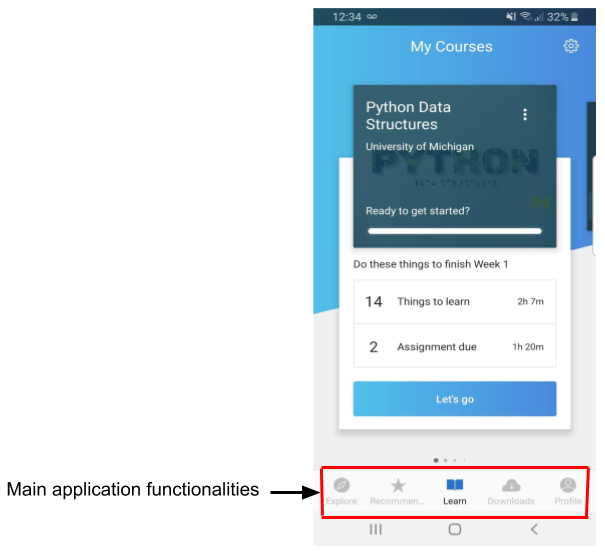
\includegraphics[scale = 0.5]{./imgs/CourseraApp}
				\caption{View of the coursera app main feature - Learn}
				\label{courseraApp}
		
			\end{figure}

		\subsubsection{Design principles}
		\myparagraph{The Tab Bar design}
		\indent
		A great way to present content to the user is to structure it into categories/items. Then create a tab containing these items (usually no more than 5) and place it at the bottom/top of the screen allowing the user to switch app content by tapping on these items. This tab bar is going to be always visible highlighting the currently active category of content. One successful app that uses this approach is Facebook and has the following bar items: News Feed, Groups, Friends, Profile, Notifications and More.  However, there are two drawbacks for this approach: i) the tab bar takes a persistent amount of screen space and ii) the tab bar can contain only  5 or 6 tab items (Nielsen Norman Group, 2015).


		\myparagraph{Hub-and-Spoke pattern}
		\indent
		The Hub-and-Spoke pattern allows the user to dive into a certain section of the app (spoke) from a central point (the hub). If the user wants to switch from one section to another it needs to go through the hub. However, an app is not limited to a single hub the designer is free to pick more hubs as he sees fit. One practical application of this pattern is in mobile operating systems like iOS/Android where home-screen represents the central point (the hub) and  applications represent the spokes. A user can launch an application but if he wants to launch another one it needs to go back to the home-screen (the hub) via home-button. This pattern helps the user achieve certain tasks faster and is also often used by webpages (Flaherty, 2018).

		\myparagraph{List design}
		\indent
		When presenting a large amount of similar data items like flights or trains between two stations it is good practice to use a \textit{list}. A list contains a series of subviews and each subview has a text, an image and maybe a quick action (e.g. a button). Each list item represents an entering point to a certain app content. Often a list is accompanied by search and filtering features (Neil, 2014).

		\subsubsection{User experience}

		Coursera's mobile app is complex and yet very easy to use. The Tab Bar design is used to enhance navigation and highlights the main sections of the app content: Learn, Downloads, Profile, Recommended and Explore. When the user swaps from one tab item to another apart from highlighting the active tab item, the whole tab bar is redimensioned and for the active item tab a tile is displayed (see Figure~\ref{tabB}). This extra element added to the Tab Bar design increases the user experience by giving more feedback to the user since not everyone has the same conceptual model about what an icon might represent.
		\begin{figure}[H]

			\centering	
			
\includegraphics[scale = 0.3]{./imgs/tabBar.jpg}
			\caption{The active tab item highlighted and its title}
			\label{tabB}

		\end{figure}

		The Learn section of the app makes use of the Hub-and-Spoke pattern. Namely,  the courses to which the learner is enrolled represent the hub and from here the learner can access one of them, namely, a spoke. Please see Figure~\ref{hS} for a visual representation of the pattern used in Coursera's app.


		\begin{figure}[H]

			\centering	
			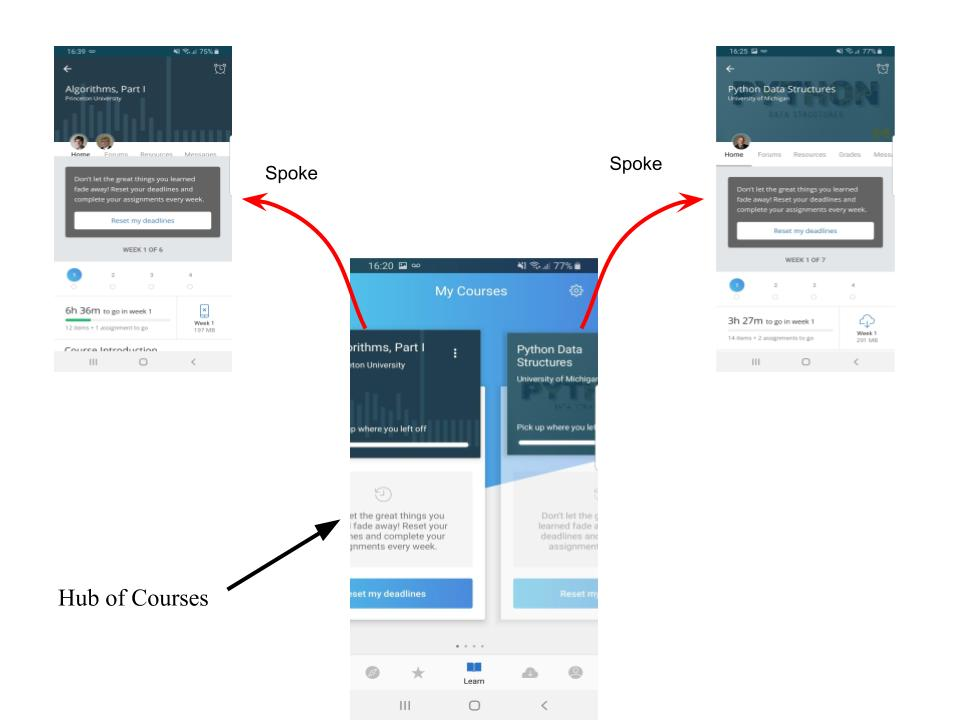
\includegraphics[scale = 0.5]{./imgs/HubSpokeCoursera.jpg}
			\caption{The Hub-and-Spoke design pattern used in Coursera's app}
			\label{hS}

		\end{figure}

	To display the catalogue of courses that the platform offers  the app makes use of an enhanced \textit{list}.  There are multiple lists that present the courses each one of them dealing with a certain category, the first element of the list representing the title of the category. The user can pan vertically to see all the available categories of courses or horizontally to see the courses under a certain category. Moreover, the courses can be filtered using  a search query. Figure~\ref{eL} presents the enhanced list used by Coursera app.

		\begin{figure}[H]

			\centering	
			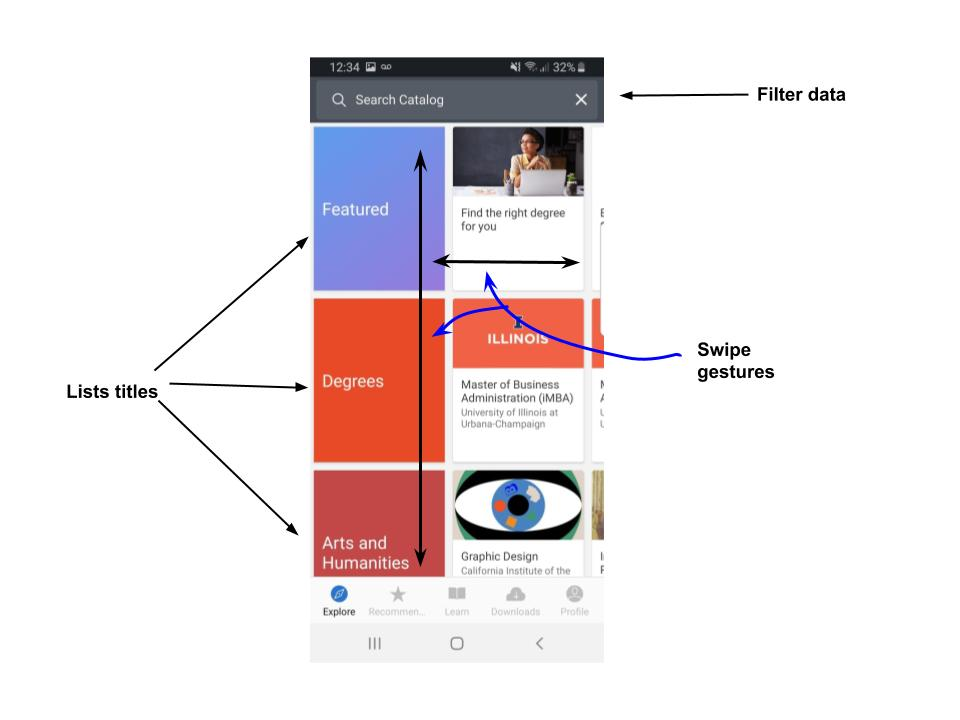
\includegraphics[scale = 0.5]{./imgs/Catalogue.jpg}
			\caption{The enhanced list design in Coursera's app}
			\label{eL}

		\end{figure}


		\subsubsection{Added value for the user}

		The application helps the user to acquire knowledge and skills regarding a certain field and complements Coursera's webpage. It increases the flexibility because now the user is not depended on an Internet connection or a computer to access the website . The largest part of the Coursera's users are professionals who have little spare time thus the application comes very handy because, for instance, they can listen to a lecture while commuting to work.  
		
		\subsubsection{Problems}
		The application has an excellent design, however, there are few things that can be improved. To mention a few of them like the course search feature does not support abbreviated query strings (e.g. University of California - UC), the next button after finishing a course section is not really visible, the course header is a bit too big taking one-third of screen space.
		
	\pagebreak
	\subsection{edX}

		\subsubsection{Purpose and target audience}		   
			The purpose of edX is to conduct research on learning and to provide as much as possible free education, naturally, the mobile application inherits these two purposes from the organization.\\

			\indent
			Being founded by two famous higher education institutions like Massachusetts Institute of Technology and Harvard University, edX learning materials are university level, thus the target audience is people who possess at least high-school knowledge.

		\subsubsection{Functionality}
			The apps' content is structured in 3 main features: Courses, Programs and Discovery.

		\myparagraph{Courses}
		\indent
			This feature presents all the courses to which the user is enrolled and is the first screen of the app (launch screen). Each course has a dedicated screen with the following sections: Lectures, Videos, Discussion, Important Dates, Handouts and Announcements. Course material is comprised of videos with transcripts that allow the user to jump to different parts of the video, lecture slides, assignments, questionnaires and/or source code for programming courses. Moreover, the videos of a course are available for download so that they can be consulted in offline mode.

		\myparagraph{Programs}
		\indent
			This feature presents all the programs to which the user is enrolled (often when one enrolls to a course it is automatically enrolled in the program which contains that course). For each programme the user is informed how many courses he has finished, how many are in progress and how many are left and the institution which has created it. If the user wishes he can pay to be evaluated and eventually obtain a certificate for the programme.


		\myparagraph{Discovery}
		\indent
		This feature lets the user  search new content for learning that might be courses, programmes or degrees. The browsing activity is supported by many filtering options.

		\subsubsection{Design principles}
		The design principles detailed in Section 1.1.3 are used by edX's mobile app, thus they will not be added in this section again.

		\subsubsection{User experience}
		The navigation between the three main features is enhanced by using the Tab Bar design. When the user swaps from one tab to another apart from highlighting the active tab the screen title is also changed. At the top of the screen, there is a set of persistent elements, namely, the profile button, the screen title and settings button. The persistent elements together with the tab bar take around one-fifth of screen space. Please see Figure~\ref{tB} to understand how the app layout looks like.

		\begin{figure}[H]

			\centering	
			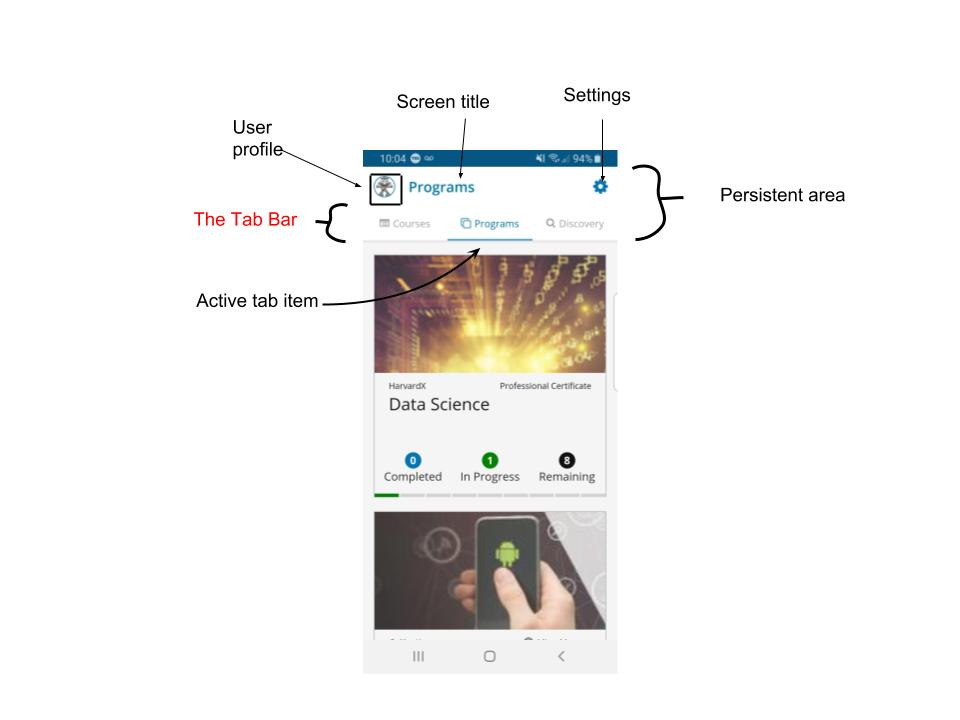
\includegraphics[scale = 0.5]{./imgs/tabBarE.jpg}
			\caption{The Tab Bar design used in edX's mobile app}
			\label{tB}

		\end{figure}

		The edX's app makes extensive use of the list design (see Figure~\ref{eU}), the design is used to present courses, programmes and degrees. However, each type of list has a custom list item layout:
		\begin{itemize}
			\item a list course item  contains: cover photo, title, course end date
			\item a list programme item contains: cover photo, programme title, institution and progress information
			\item a list degree item contains: cover photo, degree title and short bullet points of information
		\end{itemize}

		Nonetheless, the author believes that the cover photo of  the list items clutters the interface and takes too much valuable screen space and they should be resized if not removed.

		\begin{figure}[H]

			\centering	
			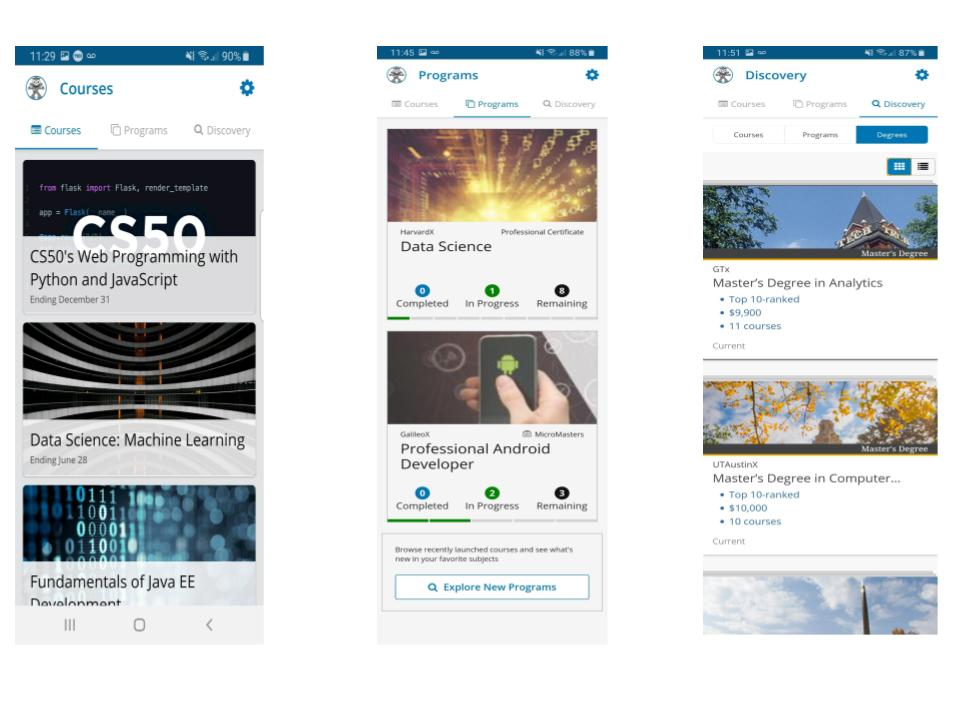
\includegraphics[scale = 0.4]{./imgs/Lists_edX.jpg}
			\caption{Extensive use of List design in edX app}
			\label{eU}

		\end{figure}

		The Hub-and-Spoke design pattern is used in edX app also. Basically, each type of list  presented in Figure~\ref{eU} acts as a hub. For instance, the course list to which the user is enrolled is a hub and from here the user can access a course (is taken to a different view) that represents a spoke (see Figure~\ref{hsE}).

		\begin{figure}[H]

			\centering	
			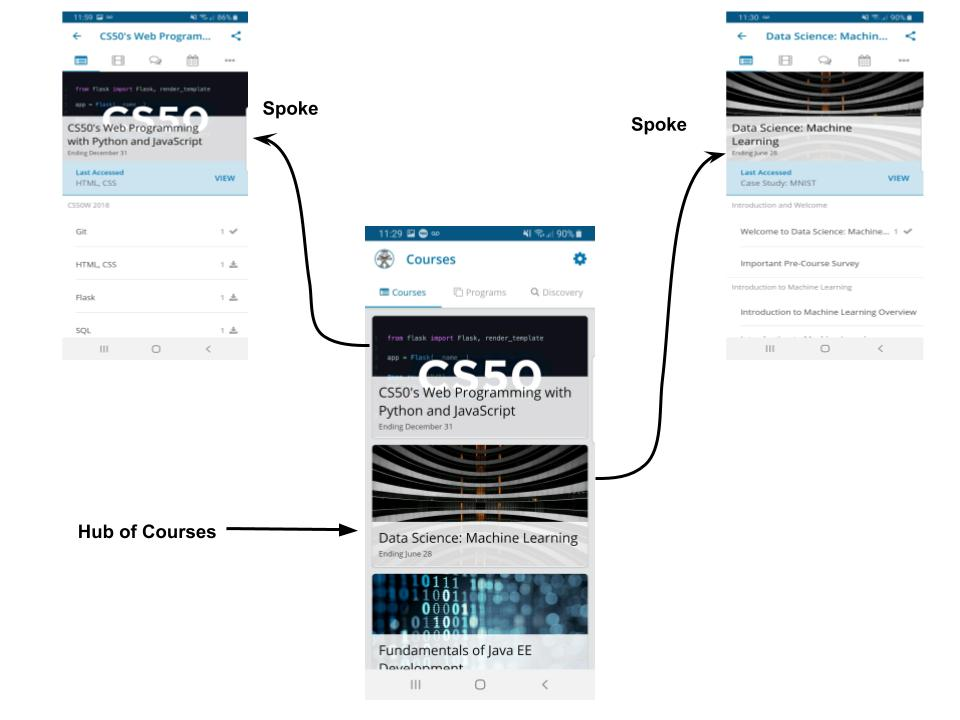
\includegraphics[scale = 0.4]{./imgs/hubAndSpokeEdX.jpg}
			\caption{The Hub-and-Spoke pattern in edX app}
			\label{hsE}

		\end{figure}

		\subsubsection{Added value for the user}
		The edX app complements the web experience provided by edX and helps the user to acquire new skills and knowledge. The app also is better suited to students because it provides a lot of courses for free and they are self-paced (the study materials available all the time). 

		\subsubsection{Problems}
		While the application contains mostly native elements, some screens are just containers for the  corresponging webpages therefore the user experience is decreased (e.g. the screens for the degrees are webpage containers). Another problem from the perspective of the design is the fact that the active tab bar item and the screen title display the same information (i.e. the text appears twice), thus it becomes redundant.\\

		The applications were tested on an Android smartphone and an iOS tablet. Overall, the author believes that Coursera app has a better design than edX app that is consistent both on smartphone and tablet. However, this fact is reasonable since Coursera is a for-profit organization and users have higher expectations when they pay for a product whereas edX is non-profit and provides many of its courses for free.

		

		%the content title is displayed twice - it takes screen space
		%placing the logo there just clutters the interface

\newpage

\section{App prototype Design}
	\subsection{App purpose and target audience}
		The app purpose is to bring education closer to the user, right in his pocket. It is important that people around the world have access to quality educational materials because nowadays the job market is looking for the educated individuals. \\
		\indent
		The target audience is all those who want to learn, whether they are high-school students or professionals looking for career advancement. 

	\subsection{Functionality}

	\myparagraph{Learn feature}
	\indent
	The app allows the user to access course materials, track his progress on each individual course, be notified when deadlines for assignments are due. For each taken course the user can listen to lecture recordings, watch lecture videos, take notes and complete questionnaires or submit solutions to exercises through the mobile application. The course materials are structured on weeks and for each week the work required is roughly the same (see Figure~{lI}). \\
	Each course provides basic information about the qualifications of the instructors so that the user knows who has created a certain course. Often the user might have questions regarding the concepts presented in a course, thus, the application provides a forum where questions can be put; a mean for the learners to interact with one another and a place where instructors can provide answers available to all the learners. Upon finishing a course the learner can receive a certificate, thus there is a need to evaluate the learner, this is done by grading each week's assignment. The app has a section for each course called \textit{Grades} where the learner can consult the marks received (see Figure~\ref{fG}). 

	\myparagraph{Explore feature}
	\indent
	This feature allows the user to browse the catalogue of courses provided by the app. The app allows courses to be filtered according to their level of difficulty, the courses are classified on the following levels: \textit{introductory, intermediate} or \textit{advanced}. Moreover, other filtering options are \textit{paid} or \textit{free}  and the possibility to add also a query string to the search action (see Figure~\ref{fG}).	

	\myparagraph{Profile}
	\indent
	The profile feature allows the user to manage settings about the app and his account information (see Figure~\ref{pE}). For instance, one can choose to disable the notifications or change the language of the application (the names of the user interface elements will be changed accordingly).\\

	\indent
	The design principles used to develop the prototype are the Tab Bar, the Hub-and-Spoke pattern and the List design. These principles are validated by their use in state-of-the-art apps like Coursera, edX and others.

	\subsection{App prototype screens and user experience}

	The home screen presents the courses to which the user is enrolled. The course information is displayed in a list item and contains  course title, instructors' university, end date and a coursework progress estimation (see Figure~\ref{hSP}). The navigation between the different sections of the app is ensured through the use of the tab bar design with following tab items: home, explore and profile. The tab bar is placed at the bottom of the each screen the app contains. 
		\begin{figure}[H]

			\centering	
			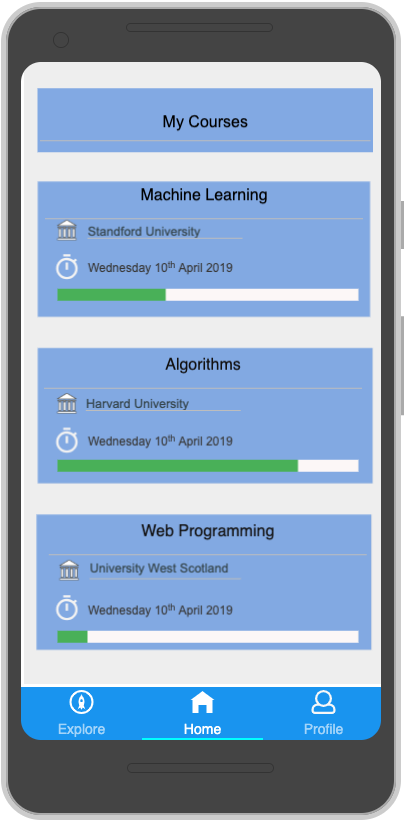
\includegraphics[scale = 0.4]{./imgs/prototype/homeScreen}
			\caption{The design of home screen of prototype app}
			\label{hSP}

		\end{figure}

	The home screen also makes use of the Hub-and-Spoke pattern. In other words, all the courses displayed in the home screen are basically a  hub from which the user can navigate to one of them (a spoke). In the Figure~\ref{lI} and Figure~\ref{fG} it can be seen how the screens associated with a course look like. All these screens make extensive use of the list design, every screen having a particular type of list. The lists however have a simplistic design (no photos as the one's in edX have) since the author believes that it helps the user to find meaningful information faster.\\

	To design the app prototype the author has used an online software available at \textit{proto.io}. The prototype app can be tested using a browser and it 

		\begin{figure}[H]

			\centering	
			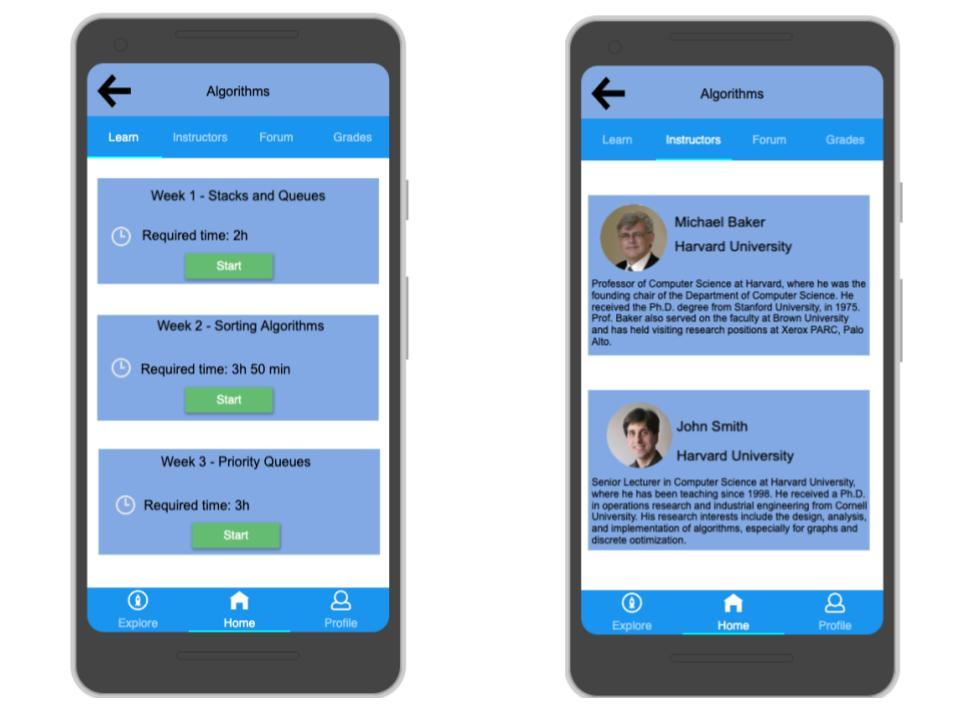
\includegraphics[scale = 0.45]{./imgs/prototype/learn+instr}
			\caption{The design of learn and instructors tabs of a course}
			\label{lI}

		\end{figure}

		\begin{figure}[H]

			\centering	
			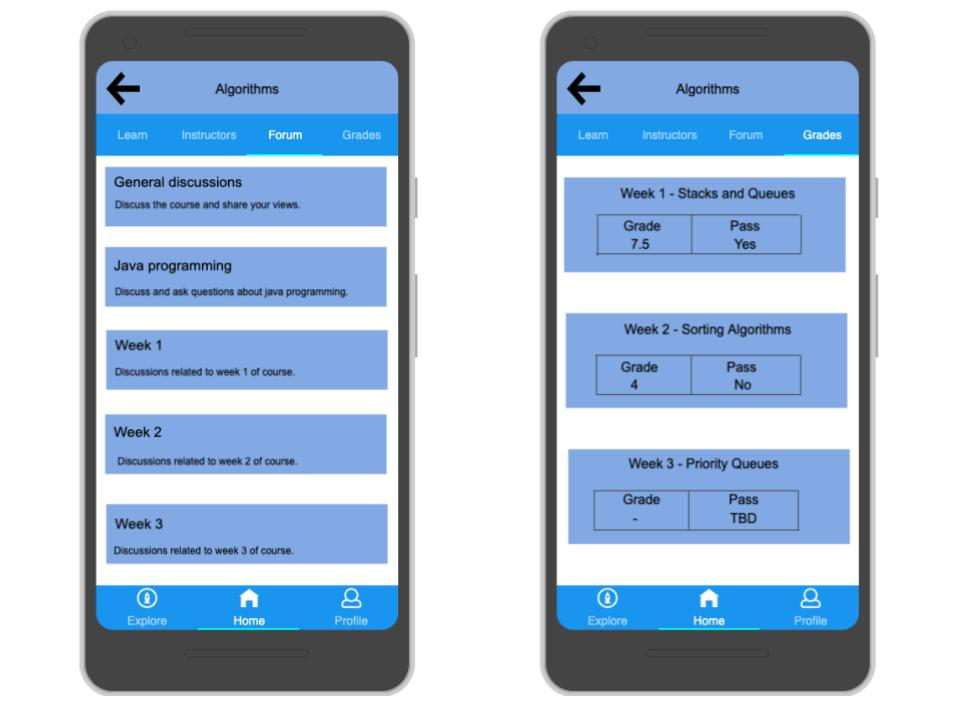
\includegraphics[scale = 0.45]{./imgs/prototype/forum+grades}
			\caption{The design of forum and grades tabs of a course}
			\label{fG}

		\end{figure}

		\begin{figure}[H]

			\centering	
			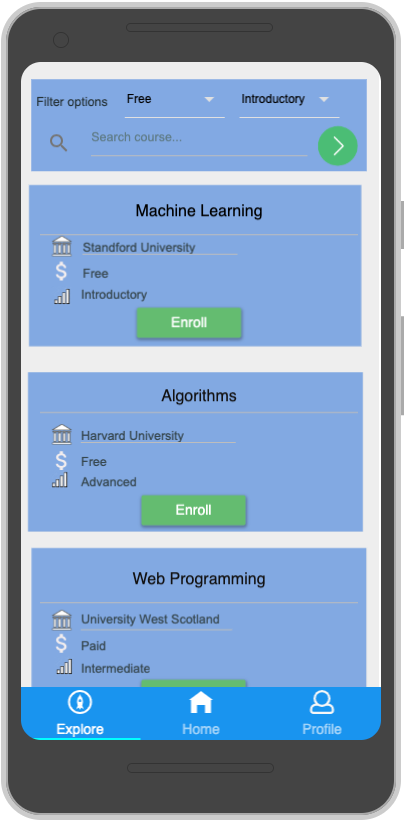
\includegraphics[scale = 0.45]{./imgs/prototype/exploreSc}
			\caption{The design of explore screen of prototype app}
			\label{fG}

		\end{figure}

		\begin{figure}[H]

			\centering	
			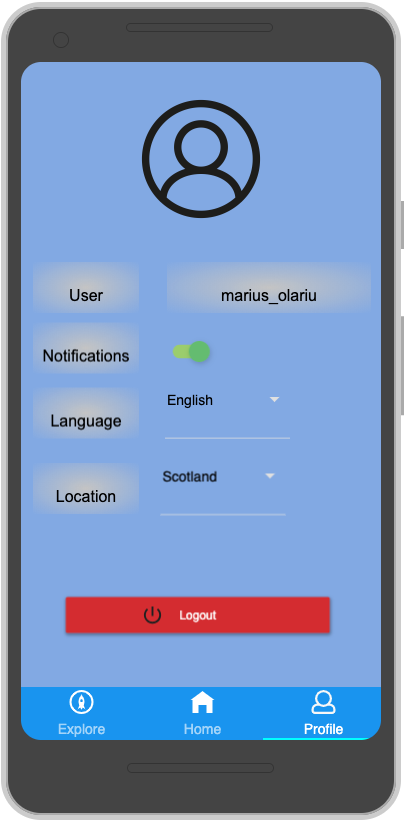
\includegraphics[scale = 0.45]{./imgs/prototype/profileSc}
			\caption{The design of profile screen of prototype app}
			\label{pE}

		\end{figure}



\newpage

\section*{References}
\underline{Coursera Android app} (2014) [Online]. play.google.com. Available: https://bit.ly/Pax9bf [Accessed 7 Apr 2019].\\

Flaherty, K. (2018) \underline{Customer-Service Information on Websites: The Hub-and-Spoke} \underline{Model} [Online]  Available: https://bit.ly/2vjozh5 [Accessed 7 Apr 2019]\\

Neil, T. (2014) \underline{Mobile design pattern gallery:} \underline{UI patterns for smartphone apps}  Sebastopol: O'Reilly Media Inc\\

 Nielsen Norman Group (2015) \underline{Basic Patterns for Mobile Navigation} [Online] Available: https://bit.ly/1RpvkVo [Accessed 7 Apr 2019]\\

Samuelson, J. (2017) \underline{New mobile features: Transcripts, notes, and reminders}  [Online]  Available: https://bit.ly/2WQtmCH [Accessed 7 Apr 2019]\\

Samuelson, J., Wang, A. (2017) \underline{Going Offline: Improvements to our most popular} \underline{mobile feature} [Online] Available: https://bit.ly/2Kfd4SI [Accessed 7 Apr 2019]

\newpage

\begin{appendices}
	\section{Complete list of Coursera app main screens}



\begin{figure}[H]
\centering
\begin{subfigure}{.55\textwidth}
  \centering
		  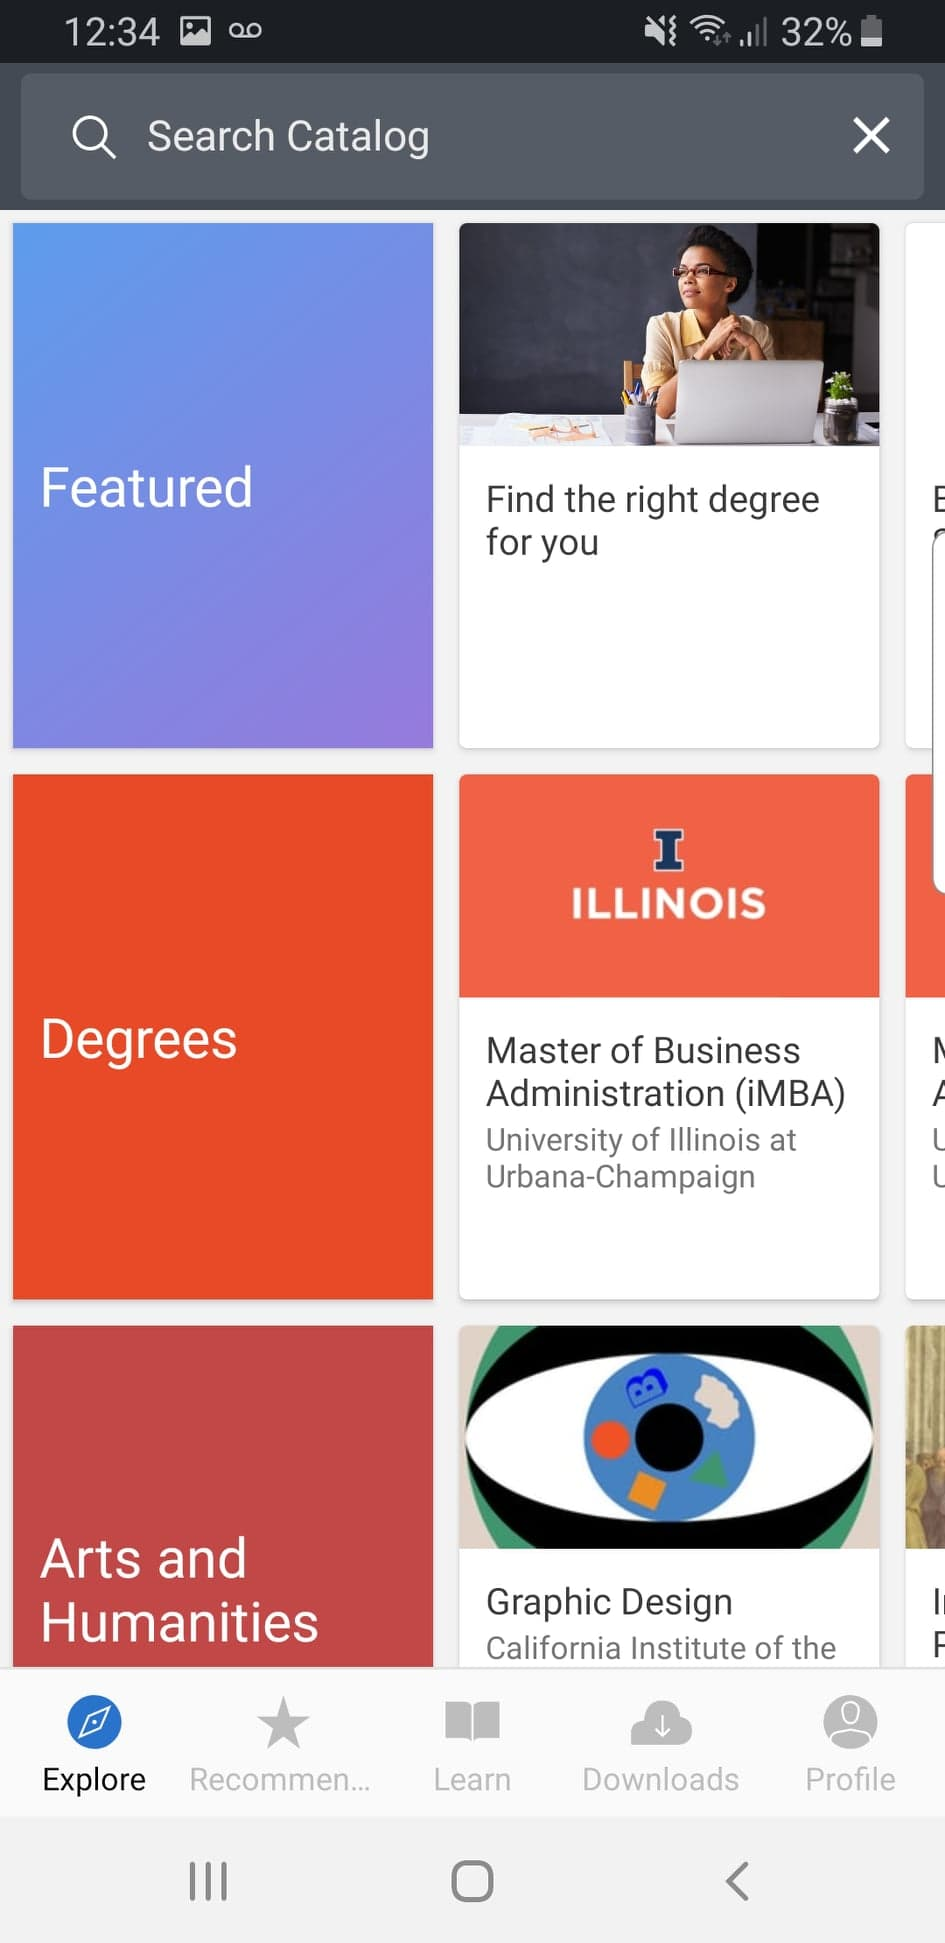
\includegraphics[width=.4\linewidth]{./imgs/exploreC.jpg}
  \caption{}{Coursera app Explore screen}
  \label{fig:sub1}
\end{subfigure}%
\begin{subfigure}{.55\textwidth}
  \centering
	  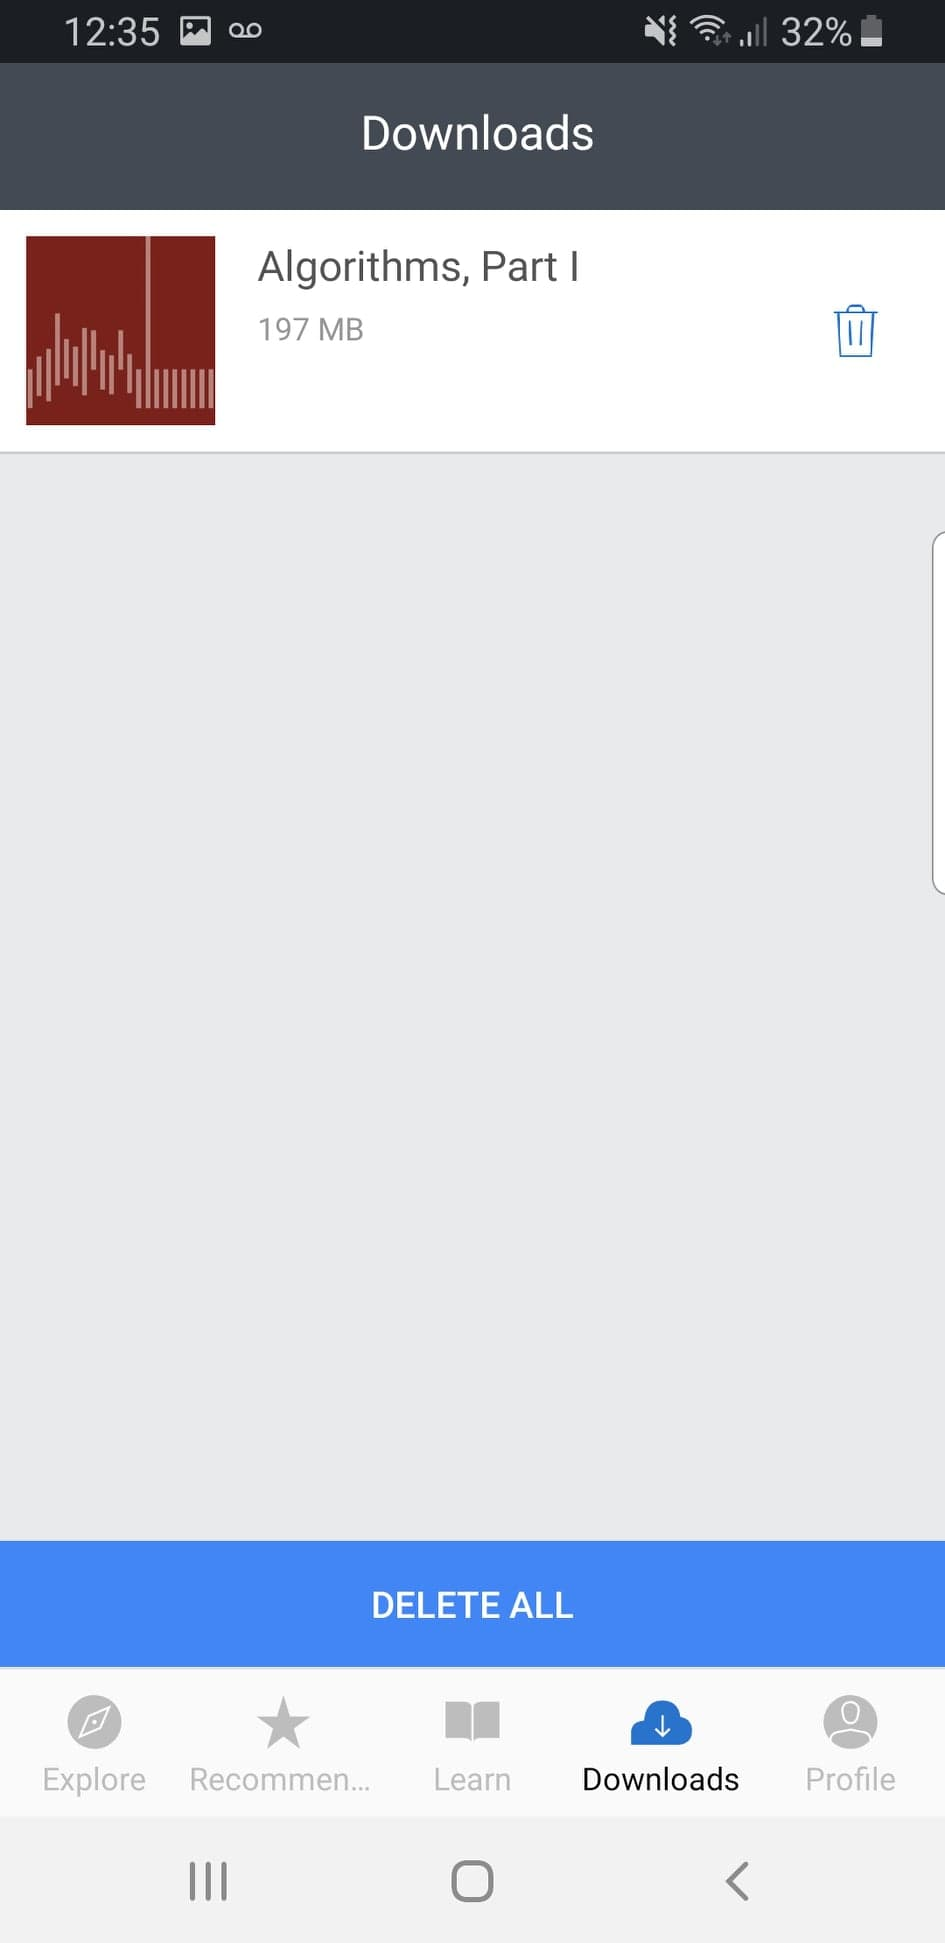
\includegraphics[width=.4\linewidth]{./imgs/DownloadsC.jpg}
	  \caption{}{Coursera app Downloads screen}

  \label{fig:sub2}
\end{subfigure}
\end{figure}

\begin{figure}[H]
\centering
\begin{subfigure}{.55\textwidth}
  \centering
		  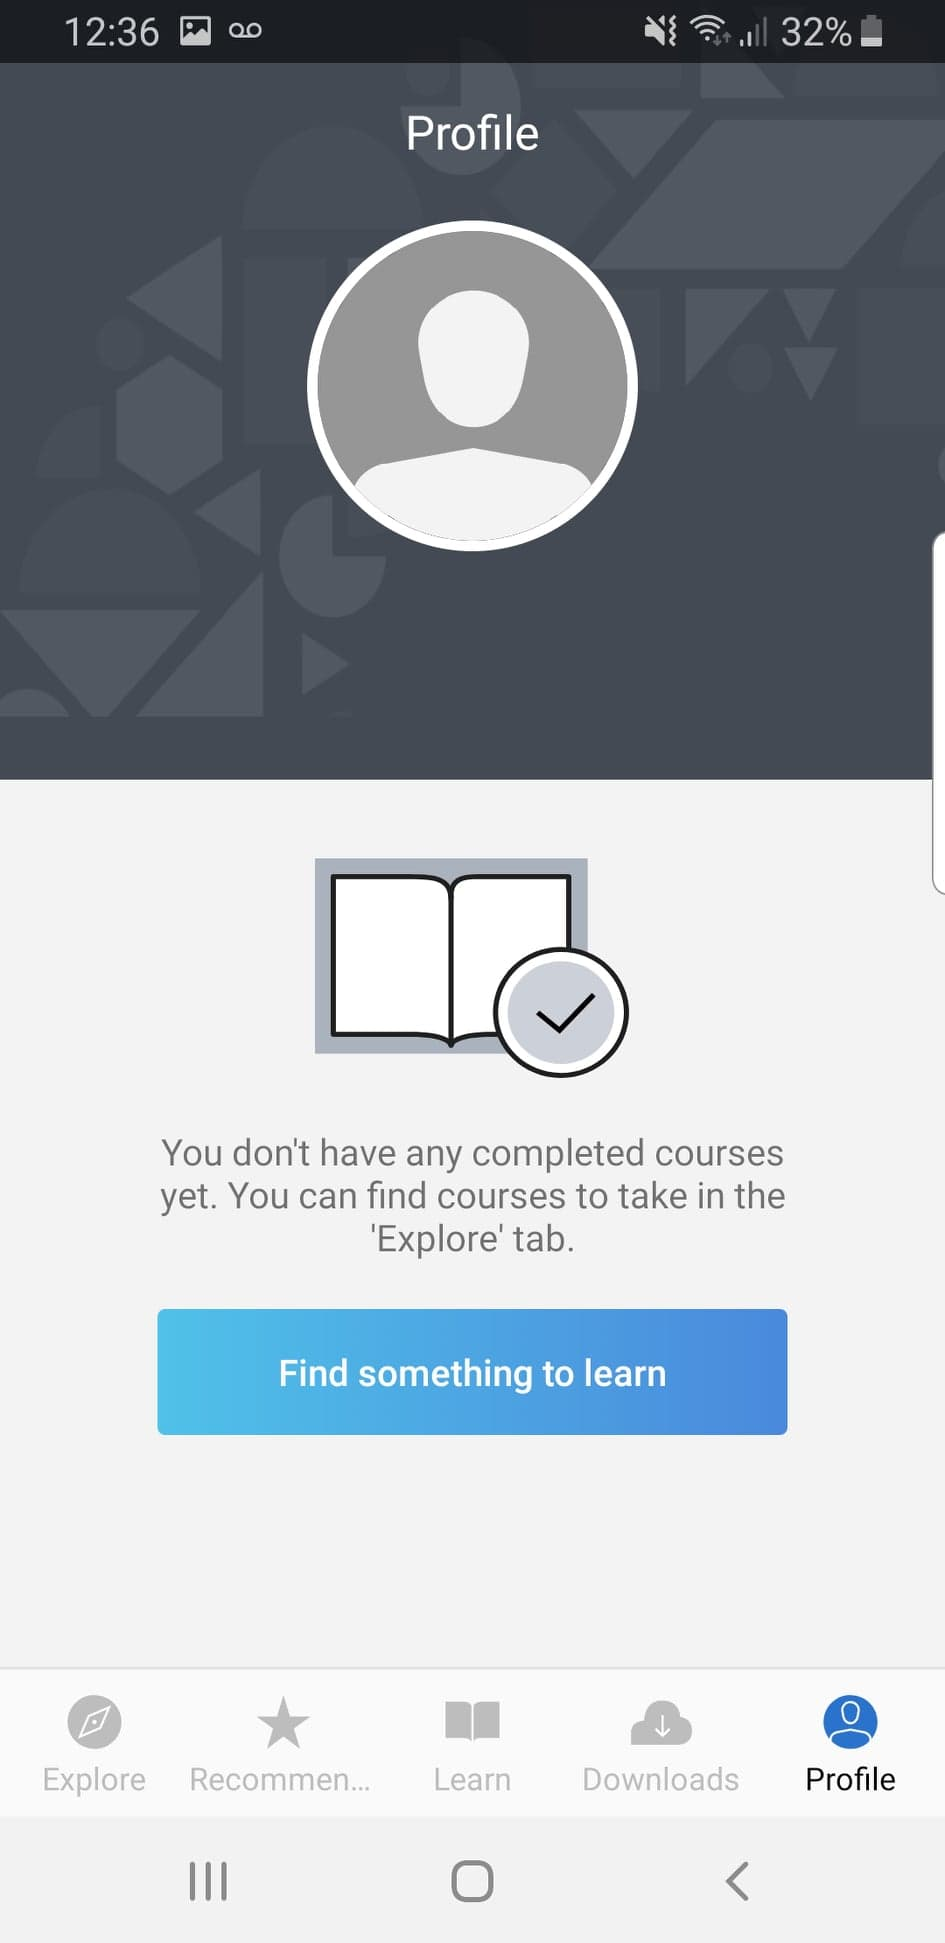
\includegraphics[width=.4\linewidth]{./imgs/profileC.jpg}
  \caption{}{Coursera app Profile screen}
  \label{fig:sub1}
\end{subfigure}%
\begin{subfigure}{.55\textwidth}
  \centering
	  
\includegraphics[width=.4\linewidth]{./imgs/recommendedC.jpg}
	  \caption{}{Coursera app Recommended screen}

  \label{fig:sub2}
\end{subfigure}

\end{figure}

			\begin{figure}

				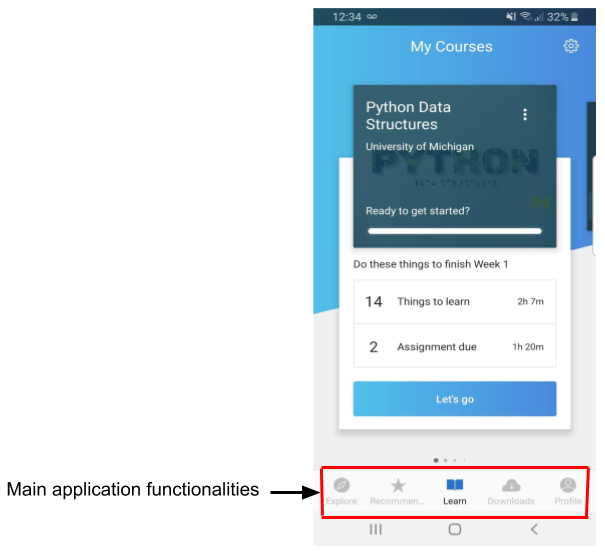
\includegraphics[scale = 0.5]{./imgs/CourseraApp}
				\caption{View of the coursera app main feature - Learn}
				\label{courseraApp2}
		
			\end{figure}


\end{appendices}


\end{document}
